\documentclass[english]{SPFShortReport}
\usepackage{subfigure}
\usepackage{spfFigures}
\usepackage{longtable}
\usepackage{url}
\usepackage{gensymb}
\usepackage[yyyymmdd,hhmmss]{datetime}
\reportName{Python calculation for heat pump SIN-8TU}
\reportSubName{Parametric Heat Pump calculation} 
\reportDate{\today \hspace{0.1cm} at: \currenttime \hspace{0.1cm} h} 
\author{Dani Carbonell}
\address{dani.carbonell@solarenergy.ch}
\begin{document}
\begin{table}[!ht]
\begin{small}
\caption{Fitted coefficients for the heat pump.}
\begin{center}
\resizebox{12cm}{!} 
{
\begin{tabular}{l | c c } 
\hline
\hline
Coefficient &Description & \\ 
 & &$[kW]$\\ 
\hline
$PQ_{1}$ & \emph{$1^{st}$ condenser polynomial coefficient}  & 7.4629e+00    \\ 
$PQ_{2}$ & \emph{$2^{st}$ condenser polynomial coefficient}  & 8.1802e+01    \\ 
$PQ_{3}$ & \emph{$3^{st}$ condenser polynomial coefficient}  & 2.4943e+01    \\ 
$PQ_{4}$ & \emph{$4^{st}$ condenser polynomial coefficient}  & -1.0992e+02    \\ 
$PQ_{5}$ & \emph{$5^{st}$ condenser polynomial coefficient}  & -1.8134e+01    \\ 
$PQ_{6}$ & \emph{$6^{st}$ condenser polynomial coefficient}  & -1.2741e+02    \\ 
\hline
$PCOP_{1}$ & \emph{$1^{st}$ COP polynomial coefficient}  & 7.3526e+00    \\ 
$PCOP_{2}$ & \emph{$2^{st}$ COP polynomial coefficient}  & 8.2053e+01    \\ 
$PCOP_{3}$ & \emph{$3^{st}$ COP polynomial coefficient}  & -1.0997e+01    \\ 
$PCOP_{4}$ & \emph{$4^{st}$ COP polynomial coefficient}  & -3.3950e+02    \\ 
$PCOP_{5}$ & \emph{$5^{st}$ COP polynomial coefficient}  & -2.6884e+00    \\ 
$PCOP_{6}$ & \emph{$6^{st}$ COP polynomial coefficient}  & -6.2924e+01    \\ 
\hline
$\dot m_{cond}$ & 1400.00 $[kg/h]$\\ 
$\dot m_{evap}$ & 1400.00 $[kg/h]$\\ 
\hline
$COP_{nom}$ (B0W35)& 4.82 \\ 
$Q_{c,nom}$ (B0W35)& 8.08 kW\\ 
$COP_{nom}$ (B2W35)& 5.12 \\ 
$Q_{c,nom}$ (B2W35)& 8.55 kW\\ 
$COP_{nom}$ (B10W35)& 6.31 \\ 
$Q_{c,nom}$ (B10W35)& 10.41 kW\\ 
\hline
\hline
\end{tabular}
}
\label{CoefTable}
\end{center}
\end{small}
\end{table}
\begin{table}[!ht]
\begin{small}
\caption{Predicting results of the heat pump.}
\begin{center}
\resizebox{12cm}{!} 
{
\begin{tabular}{l | c c c c c c c c c c c } 
\hline
\hline
$T_{evap,in}$ &$T_{evap,out}$ &$T_{cond,in}$ &$T_{cond,out}$ &$COP$ &$Q_{cond}$ &$Q_{evap}$ &$W_{comp}$ &$\dot m_{cond}$ &$\dot m_{evap}$ &$\Delta T_{evap}$ &$\Delta T_{cond}$ \\ 
$^oC$ &$^oC$ &$^oC$ &$^oC$ &$[-]$ &$[kW]$ &$[kW]$ &$[kW]$ &kg/h &kg/h &K &K\\ 
\hline
-7.00 & -10.27 & 26.05 & 30.00 & 4.07 & 6.43 & 4.85 & 1.58 & 1400 & 1400 & 3.3 & 3.9\\ 
-7.00 & -10.11 & 34.83 & 38.75 & 3.59 & 6.40 & 4.61 & 1.78 & 1400 & 1400 & 3.1 & 3.9\\ 
-7.00 & -9.74 & 43.75 & 47.50 & 2.98 & 6.11 & 4.06 & 2.05 & 1400 & 1400 & 2.7 & 3.8\\ 
-7.00 & -9.07 & 52.82 & 56.25 & 2.23 & 5.59 & 3.08 & 2.51 & 1400 & 1400 & 2.1 & 3.4\\ 
-7.00 & -7.77 & 62.03 & 65.00 & 1.31 & 4.84 & 1.14 & 3.70 & 1400 & 1400 & 0.8 & 3.0\\ 
-4.00 & -7.76 & 25.61 & 30.00 & 4.56 & 7.15 & 5.58 & 1.57 & 1400 & 1400 & 3.8 & 4.4\\ 
-4.00 & -7.58 & 34.40 & 38.75 & 3.98 & 7.09 & 5.31 & 1.78 & 1400 & 1400 & 3.6 & 4.4\\ 
-4.00 & -7.17 & 43.34 & 47.50 & 3.26 & 6.78 & 4.70 & 2.08 & 1400 & 1400 & 3.2 & 4.2\\ 
-4.00 & -6.45 & 52.43 & 56.25 & 2.40 & 6.23 & 3.63 & 2.60 & 1400 & 1400 & 2.4 & 3.8\\ 
-4.00 & -4.99 & 61.65 & 65.00 & 1.37 & 5.47 & 1.46 & 4.00 & 1400 & 1400 & 1.0 & 3.4\\ 
-1.00 & -5.25 & 25.17 & 30.00 & 5.05 & 7.87 & 6.31 & 1.56 & 1400 & 1400 & 4.3 & 4.8\\ 
-1.00 & -5.04 & 33.98 & 38.75 & 4.37 & 7.78 & 6.00 & 1.78 & 1400 & 1400 & 4.0 & 4.8\\ 
-1.00 & -4.60 & 42.93 & 47.50 & 3.54 & 7.45 & 5.34 & 2.10 & 1400 & 1400 & 3.6 & 4.6\\ 
-1.00 & -3.83 & 52.03 & 56.25 & 2.57 & 6.87 & 4.20 & 2.67 & 1400 & 1400 & 2.8 & 4.2\\ 
-1.00 & -2.23 & 61.26 & 65.00 & 1.43 & 6.09 & 1.83 & 4.26 & 1400 & 1400 & 1.2 & 3.7\\ 
2.00 & -2.74 & 24.73 & 30.00 & 5.55 & 8.59 & 7.04 & 1.55 & 1400 & 1400 & 4.7 & 5.3\\ 
2.00 & -2.51 & 33.55 & 38.75 & 4.76 & 8.47 & 6.69 & 1.78 & 1400 & 1400 & 4.5 & 5.2\\ 
2.00 & -2.04 & 42.52 & 47.50 & 3.83 & 8.11 & 5.99 & 2.12 & 1400 & 1400 & 4.0 & 5.0\\ 
2.00 & -1.22 & 51.64 & 56.25 & 2.75 & 7.51 & 4.77 & 2.73 & 1400 & 1400 & 3.2 & 4.6\\ 
2.00 & 0.50 & 60.89 & 65.00 & 1.49 & 6.70 & 2.22 & 4.48 & 1400 & 1400 & 1.5 & 4.1\\ 
5.00 & -0.23 & 24.29 & 30.00 & 6.06 & 9.30 & 7.77 & 1.53 & 1400 & 1400 & 5.2 & 5.7\\ 
5.00 & 0.03 & 33.13 & 38.75 & 5.16 & 9.16 & 7.38 & 1.77 & 1400 & 1400 & 5.0 & 5.6\\ 
5.00 & 0.52 & 42.12 & 47.50 & 4.12 & 8.77 & 6.64 & 2.13 & 1400 & 1400 & 4.5 & 5.4\\ 
5.00 & 1.39 & 51.26 & 56.25 & 2.93 & 8.14 & 5.36 & 2.78 & 1400 & 1400 & 3.6 & 5.0\\ 
5.00 & 3.22 & 60.51 & 65.00 & 1.57 & 7.31 & 2.64 & 4.67 & 1400 & 1400 & 1.8 & 4.5\\ 
8.00 & 2.28 & 23.86 & 30.00 & 6.57 & 10.01 & 8.49 & 1.52 & 1400 & 1400 & 5.7 & 6.1\\ 
8.00 & 2.56 & 32.71 & 38.75 & 5.56 & 9.84 & 8.07 & 1.77 & 1400 & 1400 & 5.4 & 6.0\\ 
8.00 & 3.09 & 41.71 & 47.50 & 4.42 & 9.43 & 7.29 & 2.13 & 1400 & 1400 & 4.9 & 5.8\\ 
8.00 & 3.99 & 50.87 & 56.25 & 3.12 & 8.77 & 5.95 & 2.81 & 1400 & 1400 & 4.0 & 5.4\\ 
8.00 & 5.92 & 60.14 & 65.00 & 1.64 & 7.92 & 3.09 & 4.83 & 1400 & 1400 & 2.1 & 4.9\\ 
11.00 & 4.79 & 23.42 & 30.00 & 7.09 & 10.72 & 9.21 & 1.51 & 1400 & 1400 & 6.2 & 6.6\\ 
11.00 & 5.10 & 32.29 & 38.75 & 5.97 & 10.53 & 8.76 & 1.76 & 1400 & 1400 & 5.9 & 6.5\\ 
11.00 & 5.65 & 41.31 & 47.50 & 4.72 & 10.08 & 7.94 & 2.14 & 1400 & 1400 & 5.4 & 6.2\\ 
11.00 & 6.58 & 50.48 & 56.25 & 3.31 & 9.40 & 6.55 & 2.84 & 1400 & 1400 & 4.4 & 5.8\\ 
11.00 & 8.60 & 59.77 & 65.00 & 1.72 & 8.52 & 3.56 & 4.96 & 1400 & 1400 & 2.4 & 5.2\\ 
14.00 & 7.31 & 22.98 & 30.00 & 7.61 & 11.43 & 9.93 & 1.50 & 1400 & 1400 & 6.7 & 7.0\\ 
14.00 & 7.63 & 31.87 & 38.75 & 6.39 & 11.21 & 9.45 & 1.75 & 1400 & 1400 & 6.4 & 6.9\\ 
14.00 & 8.21 & 40.91 & 47.50 & 5.02 & 10.73 & 8.60 & 2.14 & 1400 & 1400 & 5.8 & 6.6\\ 
14.00 & 9.18 & 50.10 & 56.25 & 3.50 & 10.02 & 7.16 & 2.86 & 1400 & 1400 & 4.8 & 6.1\\ 
14.00 & 11.27 & 59.40 & 65.00 & 1.80 & 9.12 & 4.05 & 5.07 & 1400 & 1400 & 2.7 & 5.6\\ 
17.00 & 9.83 & 22.55 & 30.00 & 8.13 & 12.14 & 10.64 & 1.49 & 1400 & 1400 & 7.2 & 7.4\\ 
17.00 & 10.17 & 31.46 & 38.75 & 6.80 & 11.88 & 10.14 & 1.75 & 1400 & 1400 & 6.8 & 7.3\\ 
17.00 & 10.77 & 40.51 & 47.50 & 5.33 & 11.39 & 9.25 & 2.14 & 1400 & 1400 & 6.2 & 7.0\\ 
17.00 & 11.77 & 49.72 & 56.25 & 3.70 & 10.64 & 7.76 & 2.88 & 1400 & 1400 & 5.2 & 6.5\\ 
17.00 & 13.93 & 59.04 & 65.00 & 1.88 & 9.72 & 4.56 & 5.16 & 1400 & 1400 & 3.1 & 6.0\\ 
20.00 & 12.35 & 22.12 & 30.00 & 8.66 & 12.84 & 11.36 & 1.48 & 1400 & 1400 & 7.7 & 7.9\\ 
20.00 & 12.71 & 31.04 & 38.75 & 7.23 & 12.56 & 10.82 & 1.74 & 1400 & 1400 & 7.3 & 7.7\\ 
20.00 & 13.33 & 40.11 & 47.50 & 5.64 & 12.03 & 9.90 & 2.13 & 1400 & 1400 & 6.7 & 7.4\\ 
20.00 & 14.36 & 49.34 & 56.25 & 3.90 & 11.26 & 8.37 & 2.89 & 1400 & 1400 & 5.6 & 6.9\\ 
20.00 & 16.57 & 58.67 & 65.00 & 1.97 & 10.31 & 5.09 & 5.22 & 1400 & 1400 & 3.4 & 6.3\\ 
\hline
\hline
\end{tabular}
}
\label{ResultsTable}
\end{center}
\end{small}
\end{table}
\begin{figure}[!ht]
\begin{center}
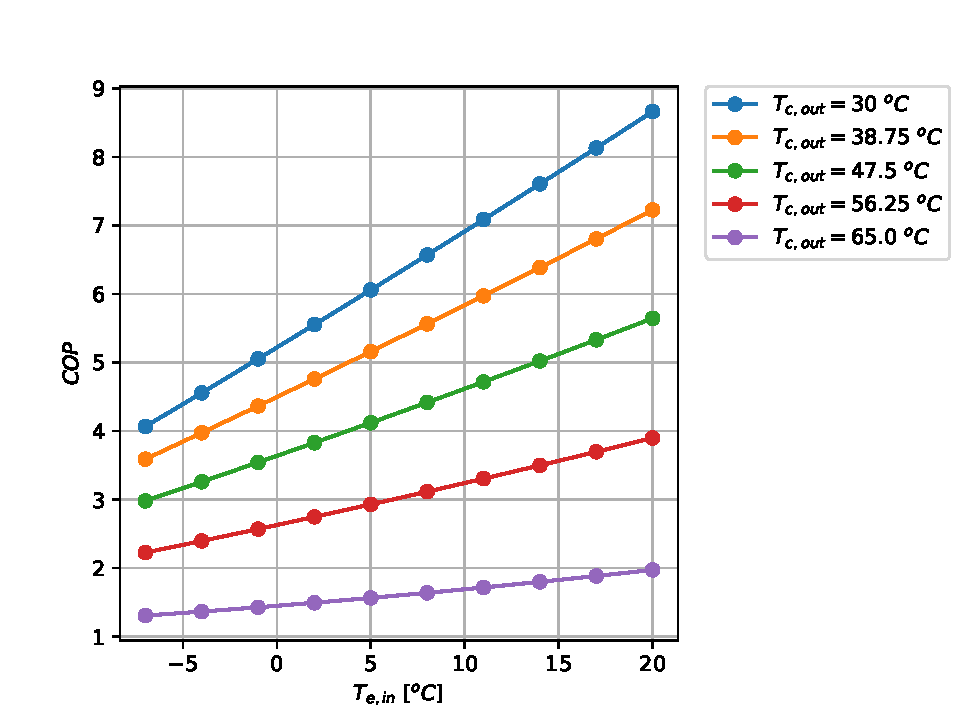
\includegraphics[width=1\textwidth]{C:/Daten/spfPackages/GIT/spfTrnsysFiles/HeatPump/BrineToWater/Walter Meier/SIN-8TU/SIN-8TU-Cop.pdf}
\caption{COP Results for the heat pump at the selected points}
\label{COPFig}
\end{center}
\end{figure}
\begin{figure}[!ht]
\begin{center}
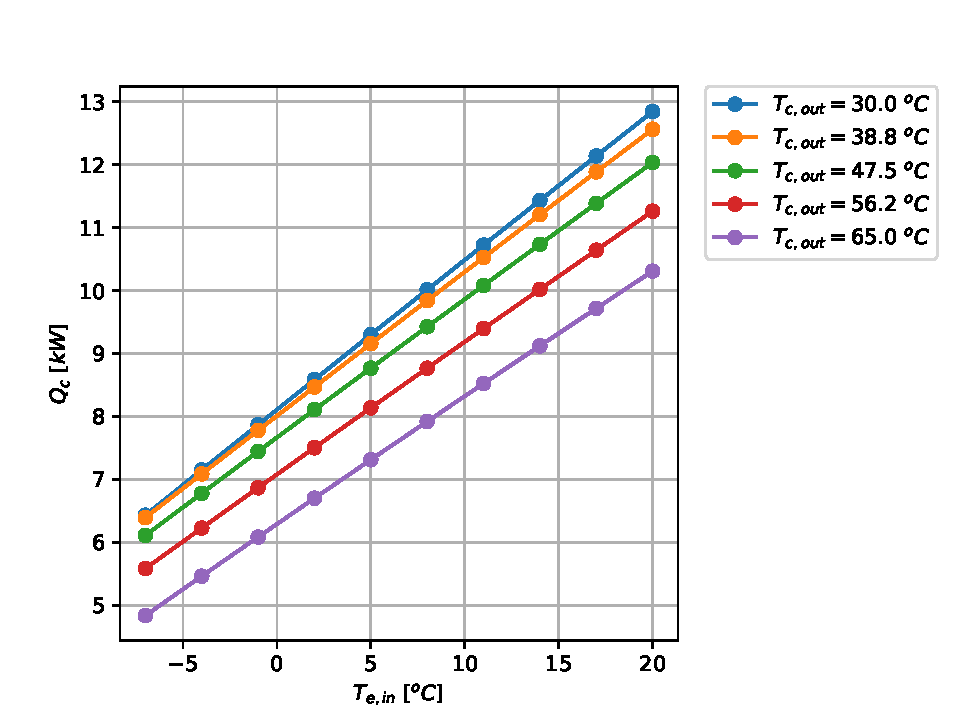
\includegraphics[width=1\textwidth]{C:/Daten/spfPackages/GIT/spfTrnsysFiles/HeatPump/BrineToWater/Walter Meier/SIN-8TU/SIN-8TU-Qc.pdf}
\caption{$Q_c$ Results for the heat pump at the selected points}
\label{QcFig}
\end{center}
\end{figure}
\end{document}
